%------------------------------------------------------------------------------
%  DOCUMENT CONFIGURATION
%------------------------------------------------------------------------------

\documentclass[twoside, a4paper, titlepage]{article}

%------------------------------------------------------------------------------
%  PACKAGES
%------------------------------------------------------------------------------

\usepackage[utf8]{inputenc}
\usepackage[english]{babel}
\usepackage{csquotes} % Recommended

\usepackage{natbib}
\bibliographystyle{agsm}

\usepackage{fancyhdr} % Required for custom headers
\usepackage{lastpage} % Required to determine the last page for the footer
\usepackage{extramarks} % Required for headers and footers
\usepackage{graphicx} % Required to insert images
\usepackage{rotating} % Required for sideways figure
\usepackage{parskip} % Required for paragraph styling
\usepackage{float} % For having figures inline
\usepackage{amsmath}
\usepackage{amssymb}
\usepackage{hyperref} % For links
\usepackage{blindtext}
\usepackage{outlines}
\usepackage{tabularx}
\usepackage{minted}
\usepackage{titlesec} % Used for paragraph subsubsubsection

\usepackage{tikz}
\restylefloat{figure}

%------------------------------------------------------------------------------

% Margins
\topmargin=-0.45in
\evensidemargin=0in
\oddsidemargin=0in
\textwidth=6.5in
\textheight=9.0in
\headsep=0.25in

% Numbering
\setcounter{secnumdepth}{4}
\titleformat{\paragraph}
{\normalfont\normalsize\bfseries}{\theparagraph}{1em}{}
\titlespacing*{\paragraph}
{0pt}{3.25ex plus 1ex minus .2ex}{1.5ex plus .2ex}

% Sans Serif Font
\renewcommand\rmdefault{cmss}

% Line spacing
\linespread{1.1}

% Images
\setlength\fboxsep{0pt}
\setlength\fboxrule{0.5pt}

\setlength\parskip{1.2em} % Space between paragraphs
\setlength\parindent{0pt} % Removes all indentation from paragraphs

% Tikz
\def\checkmark{ \tikz\fill[scale=0.4](0,.35) -- (.25,0) -- (1,.7) -- (.25,.15) -- cycle; }

%------------------------------------------------------------------------------
% TITLE PAGE
%------------------------------------------------------------------------------

\begin{document}

% Definition of blocks:
\tikzset{%
  block/.style    = {draw, thick, rectangle, minimum height = 3em,
    minimum width = 3em},
  sum/.style      = {draw, circle, node distance = 2cm}, % Adder
  input/.style    = {coordinate}, % Input
  output/.style   = {coordinate} % Output
}

\pagestyle{empty}

\newcommand{\reporttitle}{Blockchain-mediated Layered Data Access}
\newcommand{\reportauthor}{Frederick Lindsey}
\newcommand{\reportsupervisor}{Dr. William Knottenbelt}
\newcommand{\reporttype}{BEng. Individual Project Report}

\begin{titlepage}

\newcommand{\HRule}{\rule{\linewidth}{0.5mm}}

\centering % Center remainder of the page
\vspace{1cm}


%-------------------------
%	HEADING SECTIONS
%-------------------------

\textsc{\huge \reporttype}\\[1.5cm]
\textsc{\LARGE Imperial College London}\\[0.5cm]
\textsc{\Large Department of Computing}\\[0.5cm]

%--------------------------
%	TITLE SECTION
%--------------------------
\includegraphics[width = 9cm]{images/imperial_college_london_coat_of_arms}\\[0.5cm]

\HRule \\[0.4cm]
{ \huge \bfseries \reporttitle}\\
\HRule \\[1.5cm]

%--------------------------
%	AUTHOR SECTION
%--------------------------

\large
\begin{minipage}{0.5\textwidth}

\textit{Author:}\\
\reportauthor

\end{minipage}%
\begin{minipage}{0.5\textwidth}

\textit{Supervisor:}\\
\reportsupervisor

\end{minipage}

\vspace{3cm}
\makeatletter
\@date

\makeatother
\end{titlepage}


%------------------------------------------------------------------------------
% CONTENT
%------------------------------------------------------------------------------

% MOTIVATION
% CONTRIBUTIONS
% RESULTS

% APPLICABILITY
\abstract

\thispagestyle{plain}
\pagenumbering{roman}
\setcounter{page}{1}

Over the last several hundred years, the way we access and manage the world's data has radically changed. Recounting medieval times when there was little to no public record of a person's assets or information, this presents a stark comparison to today's society, where our data and identities are traded on a global market, often without our knowledge.

This thesis, and it's accompanying proof of concept, seeks to investigate a method of reinstating the ownership of personal data that was once commonplace in previous centuries, without compromising on the free flowing and global nature of communication today.

Through the use of blockchain technology and alternative cryptography schemes, I present a proof of concept implementation that allows sharing data privately without the need for a centralised intermediatary. Through a practical use of proxy re-encryption, the process of atomically re-encrypting data from one identity to another, end-to-end encryption and privacy are preserved throughout the system.


% Acknowledge those who've technically or otherwise helped with completing the project
\renewcommand{\abstractname}{Acknowledgements}
\abstract

\thispagestyle{plain}
\pagenumbering{roman}
\setcounter{page}{2}

\begin{center}
  I'd like to thank Professor William Knottenbelt and Dr. Robert Learney for their support and guidance through this project. Their support was instrumental in this project and greatly appreciated.

  I'd also like to thank Professor Chris Hankin and Dr. Melek Somai for their involvement.
\end{center}


% Set up the header and footer
\pagestyle{fancy}
\pagenumbering{arabic}
% \lhead{\docAuthorName} % Top left header
\rhead{\firstxmark} % Top right header
\lfoot{\lastxmark} % Bottom left footer
\cfoot{} % Bottom center footer
\rfoot{Page\ \thepage\ of\ \pageref{LastPage}} % Bottom right footer
\renewcommand\headrulewidth{0.4pt} % Size of the header rule
\renewcommand\footrulewidth{0.4pt} % Size of the footer rule

%------------------------------------------------------------------------------
% TABLE OF CONTENTS
%------------------------------------------------------------------------------

\setcounter{tocdepth}{4}

\tableofcontents

%------------------------------------------------------------------------------
% INTRODUCTION AND PREFACE
%------------------------------------------------------------------------------

% MOTIVATION
% OBJECTIVES
% CONTRIBUTIONS
\section{Introduction}

% - Privatisation of data
%   - Google, Facebook, NHS, Banks, retail stores (loyalty programs)
%   - Data Protection Act (limitations and corporate-focus)
% - User choice (who do I want to have my data and how)
% - Online identities
%   - Global identity tracking
%   - Conglomerate identity providers
\subsection{Motivation}

Over the last 350 years, the general public has proceeded, often unwittingly, to give up their right to privacy by exchanging personal data for the convenience of the modern world, most often in the control of corporations and conglomerates.
\newline
One might attribute the origin of this movement in the UK to the introduction of paper money by the Bank of England~\parencite{bankofengland:2016:online} in 1694. The introduction of paper currency gave an opportunity to the Bank of England to start collecting data on the exchange of money nationally. At the time it is unlikely that any person exchanging gold for paper currency was aware of this signficant social change since they were more concerned with the convenience afforded to them. Before this time, a person might have kept their savings 'under the mattress' and almost certainly would not have shared information relating to their wealth with another party. Whilst bank notes were introduced as a means to raise funds for war, inadvertently the seed for a data revolution was sewn. Whilst no unique identities were shared at this point, they would be in years to come.

Fast forward several hundred years and we find ourselves in a society where it is commonplace to rely on few key corporations and organisations to control information nationally and internationally. As what is probably the world's most popular social network it is clear from Facebook's terms and conditions~\autocite{facebookterms:2015:online} that our use of the social network is subject to a few key conditions which restrict and change the status quo of our privacy as users. Foremost, it is apparent that whilst content posted on Facebook remains the property of the owner, Facebook has the right to use it how it wishes (as per the IP license) and hence is the controller of that data. One might choose to post it on Facebook, but one cannot stop Facebook using their content without removing it from all of Facebook's services and ensuring everyone with whom one has shared it with has also removed it from Facebook. Furthermore this allows Facebook to use any content posted for machine learning, training systems and providing commercial services using the intelligence gained from the distribution of content on the Facebook network. As someone who cares for their privacy, it is my opinion that this is not an acceptable status quo.

\begin{displayquote}{
  "\textbf{When it comes to control over our own data, health data must be where we draw the line.}"~\autocite{wilbankstopol:2016:article}
}\end{displayquote}



% TODO: Swiss health identity card data

% - Privatisation of data
%   - Google, Facebook, NHS, Banks, retail stores (loyalty programs)
%   - Data Protection Act (limitations and corporate-focus)
% - User choice (who do I want to have my data and how)
% - Online identities
%   - Global identity tracking
%   - Conglomerate identity providers


At the core of the motivation for this project lay several issues corresponding to the way in which society has been manipulated over time. It is my belief that we find ourselves in the current position without any ownership of our data because we've been keen (even greedy) as a society to reap the benefits of our data without considering the longer term security effects. We have dismissed the need to care and be responsible for our data. Below, I have highlighted the key domains in which we lack control that we should have over our personal data. Whilst written as a piece of fiction, we should be aware and concerned that ignoring the social issues with data transfer allows a world to form much similar to that of George Orwell's 1984~\autocite{orwell:1984:book} - we consider the likes of corporations synonymous with that of the 'Big Brother' character.

\subsubsection{Commoditisation of personal (and private) data}

There is no doubt that search tools such as those offered by Google and Microsoft, retail stores such as those offered by Amazon, and social networks such as Facebook and Twitter, dramatically enhance our lives and give us capabilities we would never have otherwise. Often as consumers we are eager to accept these benefits without considering the means by which they are offered to us.

% TODO: Freedom to use personal data
% \subsubsection{Freedom to use personal data}



%------------------------------------------------------------------------------
% BACKGROUND
%------------------------------------------------------------------------------

\section{Background}

As a pre-face to any possible design and implementation choices, the following three sections cover revelant background material. Distributed ledger technology is considered as a means of decentralised compute. Proxy re-encryption is covered as a possible means through which encrypted data sharing is possible. Finally, possible storage solutions are covered, particularly in the context of a decentralised platform.

\subsection{Distributed Ledger Technology}

\subsubsection{Introduction to Distributed Ledger Technology}

Distributed ledger technology (DLT) is a recent invention which endeavours to make data publicly accessible through a decentralised system, providing no single point of failure. A DLT provides transparency where traditional centralised systems fall short and allows any willing and able party to be a part of the decentralised network. Furthermore, a DLT provides no easy way for any network moderator or specific party to control or override the network without the consensus of a significant number of the network's members. Combined, this technology introduces an entirely new way of dealing with transactional data and, as implemented below, any sort of data having a lifecycle.

\subsubsection{Blockchain}

The Blockchain~\footnote{\href{https://www.blockchain.com/}{Blockchain (https://www.blockchain.com)}} is the underlying technology that is used by cryptocurrencies such as Bitcoin~\footnote{\href{https://bitcoin.org/en/}{Bitcoin (https://bitcoin.org)}}. Since Blockchain was the first widely-available distributed ledger technology, most distributed ledger technologies since have chosen to adopt the blockchain name to refer to this architecture.

A traditional database is implemented such that it only maintains one current state for a given dataset~\footnote{Some databases have features allowing the user to view state (not transactions) over time (e.g. \href{https://www.postgresql.org/docs/6.3/static/c0503.htm}{PostgreSQL's Time Travel}) but these are not common and often deprecated} rather than transactions. In contrast, a blockchain, as the name would suggest, maintains a 'chain' of blocks of transactions that are agreed by the network forming a history of the chain's life. These blocks are formed of groups of transactions and are totally ordered across nodes in the network. It follows therefore that every node needs to have the entire history of the network, and that the provenance and origin of any given commodity, the unit of measure of a transaction, is maintained.

Whilst the above summarises the differences in the way a blockchain holds data compared to a traditional database, the differences in transaction ordering are far more fundamental and interesting. Consensus is used across a blockchain network to establish the most popular chain of transactions. It is possible for many chain possibilities to exist at any given time, but the longest chain is always assumed to be the main chain. Once a client has accepted a transaction (as part of a block), and it therefore forms part of their chain, it is not possible to choose another chain where this transaction has not been accepted (as part of the same block).

\subsubsection{Blockchain Consensus}

A few of the most popular methods of achieving consensus in a blockchain, and therefore total ordering, are listed below.

\begin{itemize}
  \item
    \textbf{Proof Of Work (PoW)}
    \textit{The majority of compute power in the network is held by honest members.~\footnote{Used by Bitcoin and Ethereum (pre-Serenity). \href{https://en.bitcoin.it/wiki/Proof_of_work}{Bitcoin Wiki}}}
  \item
    \textbf{Proof Of Stake (PoS)}
    \textit{The majority of stake (currency) in the network is held by honest members.~\footnote{Planned to be used by Ethereum (Serenity release and beyond). \href{https://www.cryptocompare.com/coins/guides/the-ethereum-releases-of-frontier-homestead-metropolis-and-serenity/}{Crypto Compare}}}
  % \item
  %   \paragraph{Byzantine Agreement (BA)}
  % \item
  %   \paragraph{Tendermint (TM)}
  % \item
  %   \paragraph{Stellar Consensus Protocol (SCP)}
\end{itemize}

\paragraph{Proof of Work}

Originally proposed as a method for countering denial of service attacks, Hashcash, authored by \cite{hashcash:1997:misc} and re-evaluated in \cite{hashcash:2002:online}, is the original proof of work scheme. The idea is that using cost-functions~\footnote{A cost-function should be parametrically expensive to compute, but efficiently verifiable. \cite{hashcash:2002:online}}, the hash of some $x$ is computed such that the left-most $n$ bits are equal to $0$. Since the hash of any two similar values is very different, as shown in program code \ref{code:example_keccak_unpredictability}, a cost-function designed in this way is difficult to compute.

\begin{listing}[H]
  \centering
  \begin{minted}{bash}
> hash('keccak256').update('Hello World!0').digest().toString('hex')
'2c6e6992915d52790a3625b459a0e7a1540a7770a6582f926d0119266b6f9f51'
> hash('keccak256').update('Hello World!1').digest().toString('hex')
'4d880de6488218d7153abeacff100608191ea63cccdd9894a602e8b3c959a276'
> hash('keccak256').update('Hello World!3').digest().toString('hex')
'f016006873889f59798ff191de74c0953892b38f77dbefc67b45af5ac705fcff'
  \end{minted}
  \caption{
    Variance between hashes of similar values
  }{
    Three similar values, shown to have very different hashes using the Keccak 256-bit hash function.
  }
  \label{code:example_keccak_unpredictability}
\end{listing}


As stated in the original Bitcoin paper (\cite{bitcoin:2008:misc}), the cryptocurrency uses Hashcash to provide block validation and to chain blocks of transactions together. As per Hashcash, the hash of the next (proposed) block must have the top $n$ bits set to zero. This value is how the network self-manages, adjusting $n$ according to a moving average of the number of blocks per hour. The hash of any particular block is computed by hashing the previous block's hash, the content of the block, and some nonce (a random value). As the nonce is incremented the hash of the block varies hugely and with sufficient iterations, the block will match the requirements of the next block.

Given the nonce we have a function difficult to compute but easy to verify, providing integrity to the underlying transactions, and ensuring that should any block be changed that's been verified, all child blocks (recursively) must be recomputed. If we assume that $51+\%$ of the compute power in the network is on honest nodes, then the longest chain will also be honest. Any malicious party would need to outpace the honest nodes in the network in order to take control and re-write the chain. The so-called $51\%$ attack is the most significant security threat to the proof-of-work model.

The proof-of-work model summarised above is used in the Bitcoin and Ethereum cryptocurrency systems for their main networks as of 15th June 2017.

\paragraph{Proof of Stake}

Intended as an alternative consensus mechanism to Proof of Work (PoW), Proof of Stake (PoS) uses a party's stake in the network to determine it's voting rights to the new block. This is in direct constrast to PoW which uses a party's compute power.

Neither Ethereum nor Bitcoin currently use proof of stake, although Ethereum is intending to use it in future releases. It remains a controversial consensus method, and as such is only summarised here.

As described by Ethereum~\footnote{\href{https://github.com/ethereum/wiki/wiki}{\textit{Ethereum Wiki}}}, there are two major consensus algorithms within the PoS category, \textbf{chain-based} and \textbf{Byzantine Fault Tolerance (BFT-style)}.

Within both of the major algorithms is the concept of a validator. A validator is someone who locks their ether as a deposit for a period of time. During this time, they are a current validator. In order to propose a block a party must be a current validator.

A chain-based algorithm uses a pseudo-random selection picking a current validator who is able to propose a block for a short time period. After this time period the validator changes. As in PoW the block proposed must point to some previously mined block, assuring a continuous chain is formed.

The BFT-style algorithm extends the idea behind the chain-based algorithm but over multiple rounds. In each round random validators are chosen to propose blocks. Over the rounds a consensus on a canonical block is reached, extending the chain.

% \paragraph{Byzantine}

% \paragraph{Stellar Consensus Protocol}

% \paragraph{Tendermint}

\subsubsection{Ethereum}

Ethereum extends the blockchain's uses beyond the direct exchange of currency and into the world whereby autonomous and publicly verifiable organisations and parties can live on the blockchain. By allowing the creation of so-called 'smart contracts', entities are established as part of the blockchain which can receive transactions from external parties (you and I). Through these transactions, the state of the contract is updated allowing the contract to function as a state transition system. Documentation and a Wiki page are the main sources of information on the Ethereum ecosystem~\footnote{\href{http://ethdocs.org/en/latest}{\textit{Read the Docs}, http://ethdocs.org/en/latest}}.

\paragraph{Ethereum Virtual Machine}

In the original blockchain, underpinning Bitcoin, a portion of every transaction is taken up by the script associated with performing it. In essence, this script represents the contract of the transaction. With Ethereum, the script transmitted with a transaction should be compatible with the Ethereum virtual machine (EVM). The EVM houses an environment where any conceivable computation of arbitrarily complexity can be achieved (turing-complete), with instructions authored and compiled in languages similar to JavaScript~\footnote{\href{https://solidity.readthedocs.io/en/develop/}{\textit{Solidity (Read the Docs)}, https://solidity.readthedocs.io/en/develop/}} and Python~\footnote{\href{https://github.com/ethereum/wiki/wiki/Serpent}{\textit{Serpent Wiki}, https://github.com/ethereum/wiki/wiki/Serpent}}. Through these languages contract code is compiled and 'activated' on an Ethereum network where it will be interacted with by externally-owned accounts (EOA). These interactions allow the realisation of the utility provided by the Ethereum network; the cryptographically secure underpinnings and distributed compute.

\paragraph{Decentralised Applications}

With the EVM summarised above, we move to understanding the architecture of applications hosted by the Ethereum network and run on the EVM. A decentralised application (DApp) is an application whose's logic is hosted on the Ethereum network (through the medium of smart contracts) and interacting with the logic is done through a decentralised interface.

\subsubsection{Merkle Trees}

The importance of Merkle trees in the architecture and implementation of decentralised systems cannot be underestimated. When discussing the hashing of blocks above, the hash at the core of the block is that representing the integrity value of the transactions the block contains. As will be evidenced in the discussion of decentralised storage platforms, Merkle trees are at the very core of hashing the transactions in a block.

\cite{merkle:1988:inbook} authored a scheme to build trees where the content of a node could be validated as a function of the hash of other nodes. First one chooses a suitable hash function, and applies this to all leaf nodes in a possible tree. Then, one must apply the same hash function applied to the leaf nodes to the parent nodes such that every parent's hash is the hash of the sum of it's own value and the hashes of it's direct children. This structure results in a tree as in figure \ref{fig:example_merkle_tree}.

\begin{figure}[H]
  \centering
  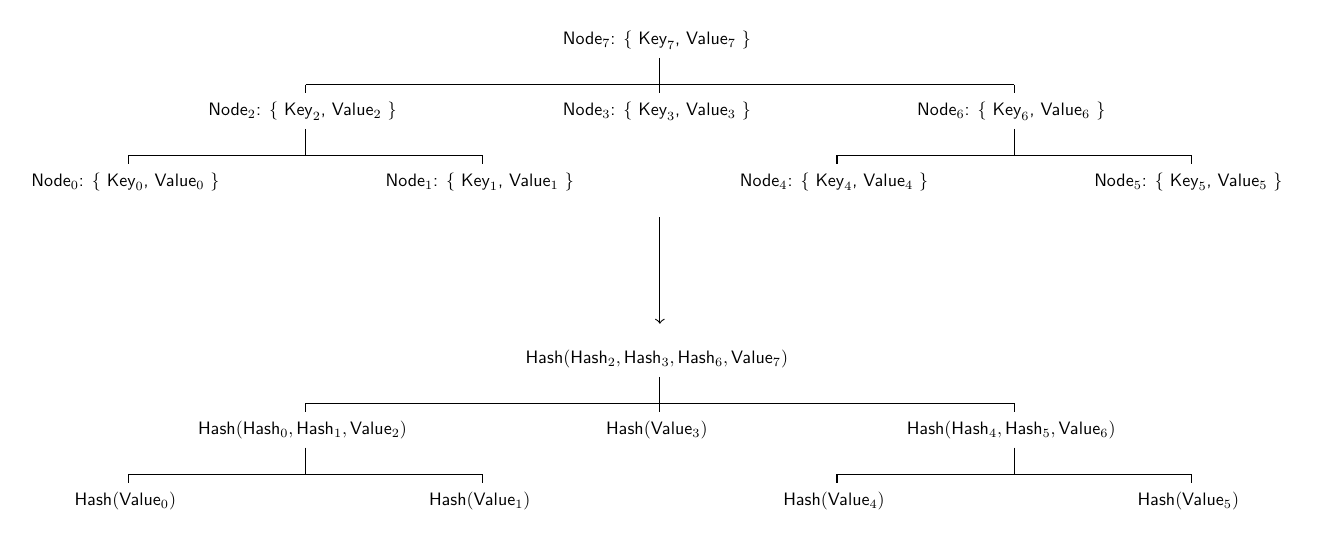
\begin{tikzpicture}[scale = 0.45, every node/.style={scale = 0.65}, every node/.append style={fill = white, rounded corners = 2pt, inner sep = 2pt, align = center}]

  \node at (0, 0) { $\text{Node}_7$: \{ $\text{Key}_7$, $\text{Value}_7$ \} };

  \draw (0, -0.5) -- (0, -1.5);
  \draw (-10, -1.25) -- (10, -1.25);
  \draw (-10, -1.25) -- (-10, -1.5);
  \draw (10, -1.25) -- (10, -1.5);

  \node at (-10, -2) { $\text{Node}_2$: \{ $\text{Key}_2$, $\text{Value}_2$ \} };
  \node at (0, -2) { $\text{Node}_3$: \{ $\text{Key}_3$, $\text{Value}_3$ \} };
  \node at (10, -2) { $\text{Node}_6$: \{ $\text{Key}_6$, $\text{Value}_6$ \} };

  \draw (-10, -2.5) -- (-10, -3.25);
  \draw (-15, -3.25) -- (-5, -3.25);
  \draw (-15, -3.25) -- (-15, -3.5);
  \draw (-5, -3.25) -- (-5, -3.5);

  \draw (10, -2.5) -- (10, -3.25);
  \draw (15, -3.25) -- (5, -3.25);
  \draw (15, -3.25) -- (15, -3.5);
  \draw (5, -3.25) -- (5, -3.5);

  \node at (-15, -4) { $\text{Node}_0$: \{ $\text{Key}_0$, $\text{Value}_0$ \} };
  \node at (-5, -4) { $\text{Node}_1$: \{ $\text{Key}_1$, $\text{Value}_1$ \} };

  \node at (5, -4) { $\text{Node}_4$: \{ $\text{Key}_4$, $\text{Value}_4$ \} };
  \node at (15, -4) { $\text{Node}_5$: \{ $\text{Key}_5$, $\text{Value}_5$ \} };

  \draw [ -> ] (0, -5) -- (0, -8);

  \node at (0, -9) { $\text{Hash}(\text{Hash}_2, \text{Hash}_3, \text{Hash}_6, \text{Value}_7)$ };

  \draw (0, -9.5) -- (0, -10.5);
  \draw (-10, -10.25) -- (10, -10.25);
  \draw (-10, -10.25) -- (-10, -10.5);
  \draw (10, -10.25) -- (10, -10.5);

  \node at (-10, -11) { $\text{Hash}(\text{Hash}_0, \text{Hash}_1, \text{Value}_2)$ };
  \node at (0, -11) { $\text{Hash}(\text{Value}_3)$ };
  \node at (10, -11) { $\text{Hash}(\text{Hash}_4, \text{Hash}_5, \text{Value}_6)$ };

  \draw (-10, -11.5) -- (-10, -12.25);
  \draw (-15, -12.25) -- (-5, -12.25);
  \draw (-15, -12.25) -- (-15, -12.5);
  \draw (-5, -12.25) -- (-5, -12.5);

  \draw (10, -11.5) -- (10, -12.25);
  \draw (15, -12.25) -- (5, -12.25);
  \draw (15, -12.25) -- (15, -12.5);
  \draw (5, -12.25) -- (5, -12.5);

  \node at (-15, -13) { $\text{Hash}(\text{Value}_0)$ };
  \node at (-5, -13) { $\text{Hash}(\text{Value}_1)$ };

  \node at (5, -13) { $\text{Hash}(\text{Value}_4)$ };
  \node at (15, -13) { $\text{Hash}(\text{Value}_5)$ };

  \end{tikzpicture}
  \caption{
    Example merkle tree
  }
  \label{fig:example_merkle_tree}
\end{figure}



\subsection{Proxy Re-Encryption}

\subsubsection{Introduction to Proxy Re-Encryption}

\begin{displayquote}{
  \textbf{"In a proxy re-encryption scheme a semi-trusted proxy converts a ciphertext for Alice into a ciphertext for Bob without seeing the underlying plaintext"}~\cite{greenateniese:2006:article}
}\end{displayquote}

Introduced as 'atomic proxy cryptography'~\cite{bbs:1998:book}, proxy re-encryption is the process of taking a message $M_a$, encrypted for a party $P_a$, and re-encrypting it such that it is readable by party $P_b$. Through the re-encryption process, the message is never decrypted by the proxy, such that the data is never revealed to any parties (including the proxy) other than the delegator and delegatees. This process relies on the functional relationship between the two ciphertexts, with the characteristics of the proxy re-encryption processed determined by the topology of this function.

\begin{figure}[H]
  \centering
  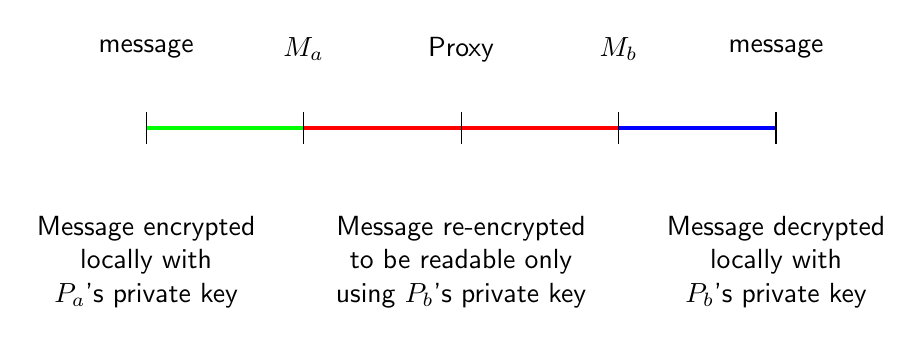
\begin{tikzpicture}

  \node at (0, 1)   {message} ;
  \node at (2, 1)   {$M_a$}   ;
  \node at (4, 1)   {Proxy}   ;
  \node at (6, 1)   {$M_b$}   ;
  \node at (8, 1)   {message} ;

  \draw [very thick, green] (0,0)   -- (2,0)   ;
  \draw [very thick, red]   (2,0)   -- (6,0)   ;
  \draw [very thick, blue]  (6,0)   -- (8,0)   ;
  \draw                     (0,-.2) -- (0, .2) ;
  \draw                     (2,-.2) -- (2, .2) ;
  \draw                     (4,-.2) -- (4, .2) ;
  \draw                     (6,-.2) -- (6, .2) ;
  \draw                     (8,-.2) -- (8, .2) ;

  \node[align=center, below] at (0, -1)%
    {Message encrypted\\locally with\\$P_a$'s private key};
  \node[align=center, below] at (4, -1)%
    {Message re-encrypted\\to be readable only\\using $P_b$'s private key};
  \node[align=center, below] at (8, -1)%
    {Message decrypted\\locally with\\$P_b$'s private key};

  \end{tikzpicture}
  \caption{
    Journey of a message using a proxy re-encryption scheme.
  }
  % \label{fig:pre_example}
\end{figure}


In figure \ref{fig:pre_example}, whether data is handled or manipulated by a fully trusted entity (a delegator or delegatee) or not is indicated using green/blue and red lines respectively.

The encrypted message $M_a$ is passed to the semi-trusted proxy along with the re-encryption key ( some $f(SK_a, PK_b)$\footnote{$SK_x$ represents the secret (private) key of a party $x$, $PK_x$ represents the public key of a party $x$.})

Below I discuss the contributions of various authors through the history of proxy re-encryption and the available schemes that might be suitable for a project focused on providing secure data sharing and storage. Specific properties of different proxy re-encryption schemes are discussed first to aid in understanding the historical context of each paper.

\subsubsection{Properties of a proxy re-encryption scheme}

\begin{table}
  \centering
  \begin{tabular}{ | l | c | c | c | }
    \hline
    Property & \cite{bbs:1998:book} & \cite{ivandodis:2003:inproceedings} & \cite{afgh:2006:article} \\
    \hline
    1. Unidirectional & & \checkmark & \checkmark \\
    2. Non-interactive & & \checkmark & \checkmark \\
    3. Proxy invisible & \checkmark & & \checkmark \\
    4. Original access & \checkmark & \checkmark & \checkmark \\
    5. Key optimal & \checkmark & & \checkmark \\
    6. Collusion 'safe' & & & \checkmark \\
    7. Temporary & \checkmark & \checkmark & \checkmark \\
    8. Non-transitive & & \checkmark & \checkmark \\
    9. Non-transferable & & & \\
  \end{tabular}
  \caption{
    \cite{afgh:2006:article} lists nine desirable properties of a proxy re-encryption scheme. Below is the table created by the author to show the benefits and compromises of the first three schemes discussed below.
  }
  \label{table:pre_properties}
\end{table}

\paragraph{Property Definitions}

\begin{enumerate}
  \item
    \textbf{Unidirectional} \\
    Creating a proxy key $\pi_{a \rightarrow b}$ allows re-encryption $A \rightarrow B$ but not $B \rightarrow A$.
  \item
    \textbf{Non-interactive} \\
    Re-encryption keys can be created with the public key from the delegatee, without the need for an authorised third party or any interaction.
  \item
    \textbf{Proxy invisible} \\
    It is not possible to determine that a proxy has re-encrypted a ciphertext. If a recipient receives a ciphertext that has been re-encrypted but is indistinguishable from a ciphertext which has only been encrypted by the recipient's public key, then the proxy has been invisible.
  \item
    \textbf{Original access} \\
    The delegator of some ciphertext retains the ability to decrypt ciphertexts that have been re-encrypted for a delegatee, thereby retaining the delegator's original access rights.
  \item
    \textbf{Key optimal} \\
    The storage of secret keys remains constant with every extra delegatee.
  \item
    \textbf{Collusion 'safe'} \\
    Should the proxy and the delegatees collude, they will be unable to reveal the secret key of the delegator.
  \item
    \textbf{Temporary} \\
    The delegatee is only able to decrypt messages encrypted by the delegator through a certain time period $i$.
  \item
    \textbf{Non-transitive} \\
    The proxy alone cannot re-delegate decryption rights, i.e. there does not exist a function $f(re_{a \rightarrow b}, re_{b \rightarrow c}) = re_{a \rightarrow c}$.
  \item
    \textbf{Non-transferable} \\
    Some proxy and delegatees are unable to re-delegate encryption rights, i.e. even with $re_{a \rightarrow b}, sk_b, pk_c$ one cannot share data with another party (a non-delegatee and not the delegator). This remains an open problem for proxy re-encryption.
\end{enumerate}

\subsubsection{Atomic Proxy Cryptography}

Recognising that it is intuitive to expect any good cryptography scheme to disallow any untrusted party to re-encrypt a ciphertext, \cite{bbs:1998:book} suggests that perhaps it is desirable to allow re-encryption of a ciphertext, but only for specific delegatees. This is subject to doing so atomically, i.e. without revealing the underlying ciphertext, and without knowledge of the delegator or delegatee being exposed in the process. Conceptually this means that a delegator can encrypt once and have semi-trusted proxies re-encrypt for delegatees when desired.

Let's suppose we have a cryptography scheme whereby the following functions are observed:

\begin{itemize}
  \item $Gen(...)$: A generator of keys requiring arbitrary arguments
  \item $Encrypt(m, k)$: Allows the encryption of a message $m$ using the $k$ such that it is only decryptable by it's counterpart (or itself, if symmetric)
  \item $Decrypt(m, k)$: Allows the decryption of some encrypted message $m$ using the key $k$. Successful only if the message $m$ was encrypted (and intended for) the owner of the key $k$.
  \item $\Pi(m, rek_{a \rightarrow b})$: Allows the re-encryption of some encrypted message $m$ intended for the owner of key $a$ such that it is decryptable by the owner of key $b$.
  \item $ReGen(..., SK_a, PK_b)$: A generator of re-encryption keys requiring arbitrary arguments including keys required to decrypt
\end{itemize}

As an example, imagine you wished to share an image privately between several friends. You encrypt this image and generate re-encryption keys for your friends (delegatees). Publishing the image and the keys means any third party (including the friends themselves) are able to re-encrypt the encrypted image such that a delegatee is able to decrypt it and view it.

The importance of the re-encryption function being atomic cannot be understated. The re-encryption function $\Pi$ alters the ciphertext effectively performing $\Pi(m_a, RK_{a \rightarrow b}) = Encrypt(Decrypt(m_a, SK_a), PK_b)$. However, if $\Pi$ were not atomic, the decryption of the message $m_a$ would reveal the plaintext content of the message to the proxy.

The following trust axioms apply to proxy re-encryption (assuming perfect implementation). The latter axiom only applies to symmetric key cryptography. Since the latter axiom is an undesirable property, we seek to only use asymmetric (public-key) cryptography to maintain security (of both parties).

\begin{itemize}
  \item A (unconditionally) trusts B since B can decrypt on behalf of A
  \item B trusts A since A can calculate $SK_b$ using the proxy key and $SK_a$. (\textit{Symmetric keys only})
\end{itemize}}

Given these properties, we will assume that asymmetric cryptography is a requirement of proxy re-encryption going forward.

\cite{bbs:1998:book} also discusses the notion of active versus passive proxy schemes distinguishing whether the delegatee has to cooperate or not in the creation of the proxy key. In practice, if the delegatee's public key is made available and is the only requirement from the delegatee then the delegator can delegate without the delegatee present, but otherwise, e.g. if the delegatee's secret key is required, the delegator needs the delegatee's cooperation to generate the proxy key required. Furthermore, in consideration of the delegator and delegatee's personally-identifying information, the proxy key can be distinguished as being transparent, translucent, or opaque depending on the ability of a third party to distinguish the two public keys the proxy is re-encrypting between.

\cite{bbs:1998:book} uses El Gamal encryption~\cite{elgamal:1985:article} as the basis for the proxy cryptography scheme suggested. A brief description of the protocol follows.

\paragraph{El Gamal Cryptography}

The El Gamal scheme includes the following functions:

\begin{itemize}
  \item $Gen(..., g, Z_n^*)$: A generator of keys requiring arbitrary arguments including some $g$, a generator in $Z_n^*$, itself a finite cyclic group of order $n$. Produces some secret key $\alpha$, whereby $0 \le \alpha \le n$, and a public key $g^\alpha$.
  \item $Encrypt(m, pk)$: Takes a random number, $r \in {0..n}$. Encrypts a message $m$ using the shared secret represented by $g^a^r = k$, A's public key to some random power. Outputs the tuple $(g^r, mk \text{ mod } n)$.
  \item $Decrypt(<pk, c>, sk)$: Decrypts some encrypted message $c$ using the secret key $sk$. Successful only if the message $c$ was encrypted for the owner of the key $sk$.
\end{itemize}

It is based on the Diffie-Helman protocol and relies on the discrete logarithm problem of $A = g^a$ being difficult.

\paragraph{BBS Scheme}

Similar to the standard El Gamal scheme, the Blaze, Bleumer, Strauss (BBS) scheme uses the same parameters but uses them to different effect.

As part of key generation, we now take $n$ to be of the form $2q + 1$ with $n$ itself prime. The generator is taken as above, with the secret key $a$ in ${0..n - 1}$, i.e. relatively prime to $n$. The inverse is also required for this scheme, so $a^{-1} \text{ mod } 2q$ is also calculated. The public key (published) is calculated as $g^a \text{ mod } n$. Encryption and decryption differ slightly to the standard El Gamal scheme:

\begin{itemize}
  \item $Encrypt(m, pk)$: Takes a random number, $r \in Z_{2q}^*$. Encrypts a message $m$ using the shared secret represented by $g^r = k$, A's public key to some random power. Outputs the tuple $(pk^r \text{ mod } n, mg^r \text{ mod } n)$.
  \item $Decrypt(<pk, c>, sk_a)$: Decrypts some encrypted message $c$ using the secret key $sk_a$. Successful only if the message $c$ was encrypted for the owner of the key $sk_a$, A. Uses the inverse of the secret key to yield $(pk^r \text{ mod } n)^{a^{-1}} = g^r (\text{mod } n)$. Taking the inverse of this result, we have the decryption key for the ciphertext: $mg^r \text{ mod } n(g^r (\text{mod } n))^{-1} = m$
\end{itemize}

Noting that the actual message is encrypted with some random $r$, this acts as a symmetric key during the encryption / decryption process. When the public key of the recipient is raised by $r$, this yields a result which is only decryptable by the intended recipient. Therefore we need a (proxy) function which is able to achieve the following:

$$
\begin{align}
& f(pk_a^r \text{ mod } n, re_{a \rightarrow b}) & &=& pk_b^r \text{ mod } n \\
\implies & f((g^a)^r \text{ mod } n, re_{a \rightarrow b}) & &=& (g^b)^r \text{ mod } n \\
\implies & re_{a \rightarrow b} & &=& g^{a^{-1}} \times g^{b}
\end{align}
$$

Note that the re-encryption process is more efficient than first decrypting the data and then re-encrypting the data with another key, since only one, atomic, exponentiation is required.

Given the reencryption key shown above ($g^{a^{-1}} \times g^{b}$), bilateral trust is required. $A$ can learn $B$'s key and vice versa. This is not desirable for this project and so we must look for alternative schemes which do not have this issue.

\subsubsection{Proxy Cryptography Revisited}

\cite{ivandodis:2003:inproceedings} suggested improved schemes which aim to address shortcomings of the original BBS scheme in their paper \textit{Proxy Cryptography Revisited}.



\subsubsection{Improved Proxy Re-encryption Schemes with Applications to Secure Distributed Storage}

\cite{afgh:2006:article} offers another take on proxy re-encryption comparing previous schemes and offering improvements.

\subsubsection{Unidirectional Chosen-Ciphertext Secure Proxy Re-Encryption~\cite{lv11:2011:article}}


\subsection{Off-chain storage}

Whilst the storage of data is well researched, since the aim of this project is to evaluate the applicability of new and immature software to solve key social and technological challenges, there is an opportunity to discover up and coming technology in the storage space.

When using blockchain as the central data lake for an application, we must consider where we store the data that it references. Whilst is is possible to store data on blockchain itself, it is impractical and extremely expensive. Storing data on the chain, assuming a transaction will be accepted on Ethereum with a gas price of 0.2 microether, at the current prices~\footnote{\$244.96 / ETH as of 4th June 2017.}, correlates to a cost of 263,023.8 USD per GB (given the transaction costs authored by \cite{cryptocompare:2017:online}).

$$
\begin{aligned}
5 * 1024^{3} * 0.2 * 10^{-6} &=& 1,073.74 \text{ ETH (2 d.p.)} \\
&=& 263,023.80 \text{ USD (2 d.p.)}
\end{aligned}
$$

Bear in mind that I have ignored other transaction costs, including submitting and storing execution cycles, and indeed a limit on block size exists on Ethereum~\footnote{\href{https://ethstats.net/}{EthStats} showed a gas limit of the order of 4.7 million as of 5th June 2017.}. Henceforth it is trivial that it would be inappropriate to store any data on blockchain other than that which represents state of the application.

To solve this issue, we therefore need to assume that data needs to be stored by some other manner such that it is readily available, but only addressed (not stored) in blockchain. Below are two solutions.

\subsubsection{Centralised data storage}

There are many incumbents in the data storage market offering centralised, redundant data platforms. The most popular at the time include \href{https://aws.amazon.com/s3/}{Amazon Web Services S3}, \href{https://cloud.google.com/storage/}{Google Cloud Storage}, and \href{https://azure.microsoft.com/en-gb/services/storage/}{Microsoft Azure Storage} to name a few. Whilst the specific storage prices for each service are not relevant, each provider offers the storage at a rate of the order of 0.01 USD / GB / month. Even if we imagine that the storage offered by Ethereum would remain persistent and accessible for fifty years, the cost of storage on modern centralised data storage platforms is of the order of more than forty thousand times cheaper.

It is not within the scope of this report to consider the performance benefits of different cloud providers and their individual architectures. None of the big players in the centralised data storage market offer similarly performant decentralised solutions that would be useful in the context of this project.

\subsubsection{Decentralised data storage}

Decentralised storage, using peer-to-peer networks for data flow, represents an interesting and novel approach for data storage. Until recently, the only commonly used peer-to-peer data storage was that of torrents. Some software providers~\footnote{Canonical provide images of their Ubuntu operating system available through torrent files. \href{https://www.ubuntu.com/download/alternative-downloads}{Ubuntu Alternative Downloads}} have made free software available through this medium before, although historically the use of torrents for mainstream content sharing has been limited to illegal activities largely involving the use of copyrighted material.

In more recent times, more modern implementations of peer-to-peer storage have arisen. The Inter-planetary File System~\footnote{IPFS is aiming to replace HTTP as the protocol we use to access data. \href{https://ipfs.io/}{\textit{IPFS is the distributed web}}} (IPFS) and Storj~\footnote{Storj aims to provide a decentralised and encrypted platform for sharing data. } are two options that somewhat extent the concept of peer-to-peer sharing through torrenting.

\paragraph{IPFS}

IPFS takes the peer-to-peer nature of torrenting and wraps it in a application and caching layers to provide a high-performance decentralised storage solution with the following benefits.

\begin{itemize}
	\item
    	\textbf{Content-based addressing} \\
        All content sent to the IPFS network is addressed as part of a Merkle tree (tree of hashes) such that the integrity of the content can be validated by the hash, and that the hash (address) remains constant with the content.
    \item
    	\textbf{Local storage of data (content)} \\
        An IPFS node caches hashes which are requested such that it can provide them more quickly to nearby peers including repeated requests by the owner of the node for the same hash.
    \item
    	\textbf{Permanent Web} \\
        Due to the decentralised nature of IPFS, and the above content-based addressing, once a blob is present on the network, it cannot be revoked without all nodes which hold a copy deleting it. For content which has not yet been requested by any other node than the one where it was created, deletion might be possible, but it should be considered that IPFS represents somewhat permanent storage.
    \item
    	\textbf{Offline Web} \\
        IPFS provides the means for offline, localised websites and storage. Rather than requiring the backbone of the internet to provide connectivity between peers, local area networks of IPFS nodes are able to communicate and share data without barriers.
\end{itemize}

\paragraph{Storj}

Pronounced 'storage', Storj leverages a cryptocurrency backbone to provide a market for storage. There are two types of users, farmers and consumers. Farmers hold chunks of data on behalf of consumers for a monthly premium, with Storj managing the geolocation of that data to ensure it's security. Storj represents what a future implementation of this project might look like in future. However, Storj only allows accessing content you own. There is no facility to share content.

Storj will not be relevant to the implementation of this project given its developed underpinnings (as a cryptocurrency) and lack of control over sharing.



%------------------------------------------------------------------------------
% DESIGN
%------------------------------------------------------------------------------

\section{Design}

\subsection{Potential Use Cases}

Before trying to design or implement anything which would meet the objectives of the project, it is useful to consider different use cases where an architecture of this nature could be beneficial. Below I have suggested a main use case and two ancillary use cases that would benefit from the architecture of this project.

\begin{displayquote}{
  "\textbf{When it comes to control over our own data, health data must be where we draw the line.}"~\cite{wilbankstopol:2016:article}
}\end{displayquote}

\subsubsection{Healthcare Data}

The notion of completely decentralised healthcare data is certainly an attractive one.

% Private data, public network
Firstly, from a security standpoint, the onus is not on any one hospital, doctor's surgery, or sub-contractor to uphold the security of a network. Since the network is public by design, all block data transferred through the network needs to be encrypted. The requirement for encryption means that the network security, in terms of data leakage, would never be upheld by a human, but by the cryptography underpinning the encryption scheme chosen.

% Decentralisation
Secondly, without the existence of a compromisable, centralised data lake, data (which mostly will exist across multiple nodes in the network) must be tampered with or removed from every location where it is stored to in fact remove or compromise it's existence in the network. On evaluation of recent global attacks, including to UK NHS hospital trusts, it is evident that providing better security of our data should always remain a high priority. Whilst encrypting our data does nothing to stop a malicious attacker from tampering with data, decentralising data such that copies are maintained in multiple locations, and ensuring that these locations are write-once prevents the tampering or compromise of existing copies of data.

% Decentralisation
Thirdly, when a patient relocates, changes their GP surgery, or moves from military to civilian health care, their previous healthcare provider is required to transfer all their data to the new provider. Should this be within the same organisation this can be problematic. However, in the scenario when a patient moves country, or when the organisation responsible for their health care changes, the transfer of data becomes much more difficult. Furthermore, should a patient wish to evaluate their health records, or share and discuss their health records with any other party, this is not possible currently. Decentralising access and control of health records is a possible solution to these problems.

Further more, for health care professionals who might be required to visit patients, the opportunity to have a local copy of data which they might need, fully cached and secured, could allow advances in treatment that are otherwise impossible whilst the requirement for internet access holds.


\subsubsection{Secured Web Data}

At current most authenticated web sessions rely on the use of usernames and passwords. Content is then sent over HTTPS providing a security layer for sensitive content. However, if an attacker can find the session id of a target, they can potentially access and use the session the user has legitimately created for illegitimate purposes.

Let's imagine there were a transport protocol whereby content was sent encrypted such that only the intended recipient would be able to decrypt the page content. Responses can then be encrypted such that the web server is the only entity able to decrypt. Responses might also contain a hash in the packet (pre-encryption) such that the content of the (signed) message can be verified by the recipient.

This transport protocol would imply that only the intended recipient (an authorised and authenticated party) would ever receive the content of a page. As a replacement for usernames and passwords, content must have come from the believed sender and content is only receivable by the intended recipient. 


\subsubsection{Fully Decentralised Messaging}

Following on from the health care use case detailed above, and of particular relevance at a time when the UK government looks to target the privacy of users online~\footnote{UK Prime minister Theresa May's suggestion of a regulated internet likely includes restrictions on the encryption of data. \href{http://www.independent.co.uk/life-style/gadgets-and-tech/news/theresa-may-internet-conservatives-government-a7744176.html}{\textit{Independent}}}, a fully decentralised, autonomous messaging system could provide a global social movement to protect the privacy of individual conversations.

As per the health care use case, being fully decentralised would be critical to the application's success. By being decentralised, no one party would have ownership of the system and it would be impossible for any one party to shutdown the system if, for example, a government requested this. For those in war-torn areas, or areas where the internet is a restricted commodity, the execution of this idea would be profound.



\input{sections/design/02_architecture}

\subsection{A Private, Access-controlled Data Sharing Platform}



%------------------------------------------------------------------------------
% IMPLEMENTATION
%------------------------------------------------------------------------------

\section{Implementation}

\input{sections/implementation/01_technology}


%------------------------------------------------------------------------------
% EXPERIMENTATION
%------------------------------------------------------------------------------

\include{sections/05_experimentation}

%------------------------------------------------------------------------------
% OPTIMISATION
%------------------------------------------------------------------------------

\include{sections/06_optimisation}

%------------------------------------------------------------------------------
% CONCLUSION
%------------------------------------------------------------------------------

\include{sections/07_conclusion}

%------------------------------------------------------------------------------
% EVALUATION
%------------------------------------------------------------------------------

\include{sections/08_evaluation}

%------------------------------------------------------------------------------
% FUTURE EXTENSIONS
%------------------------------------------------------------------------------

\include{sections/09_future_extensions}

%------------------------------------------------------------------------------
% BIBLIOGRAPHY AND APPENDICES
%------------------------------------------------------------------------------

% All sources used for research etc.
\section{Bibliography}

\bibliography{sources.bib}
% \printbibliography[heading=none]


% Appendix
\section{Appendix}

\listoflistings

\listoffigures

\listoftables

\vfill

\subsection{Program Code}

\begin{listing}[H]
  \centering
  \begin{minted}{javascript}
contract Application {

  address administrator;

  string latest;
  mapping (string => address) version_mappings;

  modifier administratorAccess() {
    if (msg.sender != administrator) throw;
    _;
  }

  modifier notExist(string version) {
    if (version_mappings[version] != 0) throw;
    _;
  }

  function Application () {
    administrator = msg.sender;
  }

  function addVersion(string version_name, address root)
    administratorAccess notExist(version_name) {
    latest = version_name;
    version_mappings[version_name] = root;
  }

  function getLatestVersion() constant returns (string, address) {
    return (latest, version_mappings[latest]);
  }

  function getVersion(string version) constant returns (address) {
    return version_mappings[version];
  }

};
  \end{minted}
  \caption{Ethereum Versioning}
  \label{code:ethereum_versioning}
\end{listing}


\begin{listing}[H]
  \centering
  \begin{minted}{python}
#!/usr/bin/env python

import secp256k1
import time
import hashlib

private_key = secp256k1.PrivateKey()

def address_comparison(iteration):
    global private_key, address
    key = private_key.tweak_add(iteration.to_bytes(32, byteorder='big'))
    key = secp256k1.PrivateKey(privkey=key)
    public = key.pubkey.serialize()
    k = hashlib.sha256()
    k.update(public)
    result = k.hexdigest()[:-20]
    return (result, address == result)

def main():
    global iterations, address
    iterations = 10000
    address = bytes(32)
    address_comparison(iterations + 1)

    start = time.time()
    for i in range(iterations):
        address_comparison(i)
    finish = time.time()

    total_time = finish - start
    print('No. of keys checked:\t' + str(iterations))
    print('Total time:\t' + str(total_time))
    print('Time per check:\t' + str(total_time / iterations))
    print('Checks per second:\t' + str(iterations / total_time))

if __name__ == '__main__':
    main()
  \end{minted}
  \caption{Python (3.5.2) script to determining key checks per second}
  \label{code:secp256k1_benchmark}
\end{listing}


\begin{listing}[H]
  \centering
  \begin{minted}{javascript}
import Web3 from 'web3'
import contract from 'truffle-contract'
import Registry from './Registry.json'
import IPFSStorage from './IPFSStorage.json'

let web3 = new Web3(new Web3.providers.HttpProvider('http://localhost:8545'))
const contractArtifacts = { Registry, IPFSStorage }
let contracts = {};
for (const k in contractArtifacts) {
  const contract_ = contract(contractArtifacts[k])
  contract_.setProvider(web3.currentProvider)
  contracts[k] = contract_
}

const accounts = web3.eth.accounts
let contractInstances = {}

async function createRegistry() {
  try {
    contractInstances.registry = await contracts.Registry.new({
      from: accounts[0], gas: 3000000, gasPrice: 10000000
    })
  } catch(err) {
    console.log(err)
  }
  return !!contractInstances.registry
}

async function createIPFS() {
  const store = await contracts.IPFSStorage.new('0x0000', '0x0000', {
    from: accounts[0], gas: 3000000, gasPrice: 10000000
  })
  return store
}

async function main() {
  const result = await createRegistry()
  const storage = await createIPFS()
  console.log('IPFS Storage created at:\t' + storage.address)
  const transaction = await contractInstances.registry.addStore(storage.address, {
    from: accounts[0]
  })
  console.dir(web3.eth.getTransaction(transaction.receipt.transactionHash))
}

main()
  \end{minted}
  \caption{
    Script to see permission-less transaction data
  }{
    Using contracts Registry and IPFSStorage as dummies, the script shows that any data sent to the chain is public and can be viewed.
  }
  \label{code:view_storage_data}
\end{listing}



%------------------------------------------------------------------------------

\end{document}
